% !TeX root = main.tex
\documentclass{./packages/informe}
\usepackage{./packages/caratula}
\usepackage[T1]{fontenc}
\usepackage[spanish]{babel}
\graphicspath{./files/src/.media/}

\begin{document} 

% caratula 
\titulo{TP 2: Recorridos y árbol generador mínimo}
\subtitulo{}
\fecha{28 de Mayo, 2023}
\materia{Algoritmos y Estructuras de Datos III}
% \grupo{Grupo 18}

\integrante{Zaid, Pablo}{869/21}{pablozaid2002@gmail.com}
\integrante{Arienti, Federico}{316/21}{fa.arienti@gmail.com}

\maketitle


% palabras clave y resumen
\addtocontents{toc}{\protect\setcounter{tocdepth}{0}}
\section*{resumen}
\addtocontents{toc}{\protect\setcounter{tocdepth}{3}}
En la teoría de grafos, el problema del \textit{árbol generador mínimo}\footnote{ Ver Thomas H. Cormen; Charles E. Leiserson; Ronald L. Rivest y Clifford Stein. Introduction to algorithms. 2009. Sección 23: \textit{Minimum Spanning Trees}.\label{foot_1}} ---o \textit{minimum spanning tree}, en inglés--- se refiere al problema de encontrar, para un grafo conexo \mbox{$G = (V,\ E)$} con función de peso $w : E \to \mathbb{R}$ asociada, un subgrafo generador conexo y acíclico de $G$ ---es decir, un árbol generador--- que minimice la suma total del peso de sus aristas.

Existen diversos métodos para la resolución de este problema. Entre ellos, los algoritmos \textit{golosos} de \textit{Prim} y de \textit{Kruskal}, que se basan en la selección de aristas de peso mínimo \textit{seguras}\footnote{ Una arista es \textit{segura} si y sólo si, al agregarla a un subgrafo de un árbol generador, el resultado sigue siendo un subgrafo de algún árbol generador.} para la construcción de una solución.  

El siguiente informe evalúa el problema de los \textit{módems}, explicado en el próximo apartado, y lo reformula como una generalización del problema del \textit{árbol generador mínimo} que aprovecha el invariante del algoritmo de \textit{Kruskal}. Además, evalúa la eficiencia de la solución propuesta de manera empírica. %en función de la aplicación de diferentes heurísticas. En particular, \textit{union by rank} y \textit{path compression}\footnote{ Ver nota al pie (\ref{foot_1}). Sección 21: \textit{Data Structures for Disjoint Sets}.\label{foot_3}}.

$\\$
\noindent Palabras clave: \textit{árbol generador mínimo, algoritmo de Kruskal}.

% \newpage

% contenido
\tableofcontents
\newpage

% introduccion
\section{El problema de los módems}\label{modems}
% el problema
El problema de los \textit{módems} que consideraremos tiene la siguiente premisa. Dado un conjunto de $N$ oficinas 
\begin{equation*}
    O := \{o_1\ ...\ o_N\}    
\end{equation*}
donde, para cada $1 \leq i \leq N$, la oficina $o_i$ se representa por su posición $(x_i,\ y_i)$ en el plano cartesiano ---cuya unidad es el metro---, queremos encontrar el costo mínimo que debemos pagar en cables UTP y de fibra óptica para conectar todas las oficinas a internet\footnote{Notar que una oficina tendrá acceso a internet si y sólo si tiene un módem o está conectada a una oficina con acceso a internet.}.

Para ello, vamos a contar con $W < N$ módems a distribuir entre las oficinas e incurriremos en un costo de $U$ o $V$ pesos, $0 \leq U \leq V$, respectivamente, por cada metro de cable UTP o de fibra óptica utilizado. Dado que los cables UTP tienen ciertas restricciones, estos se podrán utilizar si y sólo si la distancia entre dos oficinas es menor o igual a $R$ metros. 

Por ejemplo, si 
\begin{equation*}
     O = \{(0,\ 0),\ (0,\ 1),\ (1,\ 0)\},\ R = 2,\ W = 1,\ U = 1\ \: \text{y}\ \: V = 1, 
\end{equation*}
una solución podría situar al único módem en la oficina $o_1 = (0,\ 0)$ y conectar esta oficina a las restantes con un metro de cable UTP, por un costo total de dos pesos.

% modelado
\subsection{Modelado como un problema de árbol generador mínimo}\label{modelo}

Dada la descripción anterior, vamos a mostrar que el problema se puede modelar como una variante del problema del árbol generador mínimo. Lo detallamos a continuación.

Sea $G_{\text{M}}$ un grafo pesado completo cuyos vértices son el conjunto de oficinas $O$. Por cada par de vértices $u,\ v \in O$, definamos el costo de la arista $(u,\ v)$ como
\begin{equation*}
    w(u,\ v) = \begin{cases}
        d_{uv} \cdot U &\text{si}\ d_{uv} \leq R \\
        d_{uv} \cdot V & \text{si no}
    \end{cases}
\end{equation*}
%= \sqrt{(x_i - x_j)^2 + (y_i - y_j)^2}
donde $d_{uv}$ es la distancia euclideana entre ambas oficinas. Notar que $w(u,\ v)$ designa la opción más barata disponible entre un cable UTP y uno de fibra óptica. 

Luego, de haber, al menos, una oficina con un módem, $G_{\text{M}}$ modela una solución no mínima al problema de los \textit{módems} en la que todas las oficinas están conectadas entre si. 

Si $W = 1$, sigue que, para mantener a todas las oficinas conectadas y minimizar el costo empleado en los cables, basta con encontrar un árbol generador mínimo de $G_{\text{M}}$. Sin embargo, si $W > 1$, podemos reducir aún más el costo si, en vez de encontrar un árbol generador mínimo, encontramos un bosque generador mínimo de $W$ componentes conexas que sea un subgrafo de $G_{\text{M}}$. Es decir, un bosque de $W$ árboles que incluya a todos los vértices de $G_{\text{M}}$ y tenga peso mínimo.

Vamos a demostrar que este bosque es óptimo y que basta modificar al algoritmo de \textit{Kruskal}, tal que termine en la iteración $N-W$, para encontrarlo.

% optimalidad
\subsection{Demostración de optimalidad}

Supongamos, por absurdo, que un bosque generador mínimo de $W$ componentes de $G_{\text{M}}$ no es una solución óptima al problema de los módems. Luego, debe existir otro subgrafo $B \subseteq G_{\text{M}}$ cuyo peso es el mínimo posible y que, una vez dispuestos los $W$ módems, provee de internet a todas las oficinas. 

Sin embargo, $B$ también debe ser un bosque generador de $W$ componentes. Esto se debe a que: si no fuera generador, entonces no estaríamos considerando todas las oficinas en nuestro modelo; y, si no fuera un bosque de $W$ componentes, entonces podríamos reducir su peso si eliminaramos suficientes aristas ---el peso de toda arista es positivo en $G_{\text{M}}$--- hasta formar uno. Notar que tampoco puede tener más componentes, ya que no habría suficientes módems para proveer de internet a cada grupo de oficinas. 

En consecuencia, $B$ es un bosque generador de $W$ componentes conexas de $G_{\text{M}}$ que tiene un peso menor que un bosque generador mínimo de $W$ componentes  de $G_{\text{M}}$. $\rightarrow\leftarrow$ $\hfill \square$

% correctitud
\subsection{Demostración de correctitud}\label{correctitud} Vamos a demostrar primero la siguiente proposición. Dado un grafo conexo $G$, un subgrafo $B$ de un árbol generador mínimo $T \subseteq G$ es un bosque generador mínimo de $k$ componentes de $G$ si se compone de las $n - k$ aristas de peso mínimo de $T$.

\begin{proof}
Por propiedad de árboles, está claro que si $B \subseteq T$ tiene $n - k$ aristas, entonces $B$ es un bosque generador de $k$ componentes conexas. Vamos a demostrar entonces, por el absurdo, que es mínimo.

Supongamos que existe un bosque generador $B'$ de $k$ componentes de $G$ que pesa menos que $B$. Luego, podemos construir un árbol generador de $G$ tomando un conjunto $E$ de $k-1$ aristas de $T$ que unan a las $k$ componentes conexas diferentes en $B'$. Esto lo podemos hacer ya que, si tal conjunto no existierá, entonces habría, al menos, un par de vértices, ubicados en dos componentes conexas diferentes de $B'$, para los cuales no existe un camino que los una en $T$. Lo que es absurdo, dado que $T$ es un árbol generador.

Dicho esto, como estas aristas tienen, a lo sumo, el peso de las $k-1$ aristas máximas en $T$, sigue que $B' + E$ es un árbol generador de $G$ con peso menor que el árbol generador mínimo $T$. $\rightarrow\leftarrow$  
\end{proof}
En consecuencia, dado que el invariante del algoritmo de \textit{Kruskal} afirma que, para la $k$-ésima iteración, el grafo $B_k$ construido por el algoritmo es un subgrafo de un árbol generador mínimo de $G$ y, en cada iteración, el algoritmo agrega una arista segura de peso mínimo a $B_k$, para todo $1 \leq k \leq n-1$, entonces, $B_{n-k}$ es un subgrafo de un árbol generador mínimo $T$ compuesto por sus $n-k$ aristas de peso mínimo. Luego, $B_{n-k}$ es un bosque generador mínimo de $k$ componentes. $\hfill \square$

% algoritmo
\subsection{El algoritmo} Dicho todo esto, el siguiente pseudo-algoritmo presenta una solución al problema de los \textit{módems}. %que es una modificación del algoritmo de \textit{Kruskal}. 

\lstinputlisting[mathescape=true, language=pseudo, label=modems, caption={Pseudocódigo para el problema de los \textit{módems}.}]{files/src/.code/modems.pseudo}

El mismo emplea una versión modificada del algoritmo de \textit{Kruskal} que, además de terminar en la iteración $N - W$, acumula el costo incurrido en cada tipo de cable, en las variables $a$ y $b$, a medida que agrega aristas al bosque $B$. %Notar que, para el algoritmo de \textit{Kruskal}, un arista es segura si y sólo si, además de mantener su invariante, conecta a dos componentes conexas diferentes del subgrafo construido hasta esa iteración.

% complejidad
\subsection{Complejidad temporal y espacial} El algoritmo \textsc{modems} depende casi exclusivamente de la implementación del algoritmo de \textit{Kruskal} que utilicemos. Dado que el grafo $G_\text{M}$ es completo, la mejor\footnote{ En base a los algoritmos conocidos.} complejidad que podemos lograr corresponde a utilizar la implementación del algoritmo para grafos densos, cuyo costo espacial y temporal es $\Theta(n^2)$. Esta opción es teóricamente la mejor, ya que las implementaciones para grafos \textit{ralos} tienen un costo temporal en $\Theta(m\log n)$, que equivale a $\Theta(n^2 \log n)$ para este caso de uso.

%\newpage

% resultados
%\vspace{2em}
\section{Evaluación empírica}
%\vspace{1em}
%La implementación comentada del algoritmo de Kruskal parece eficiente cuando se trata de grafos ralos pero resulta menos que satisfactoria cuando se trata de estructuras más densas. En particular en este problema, se están ordenando $O(n^2)$ aristas a pesar de que solo se observan $n-1$ de ellas como máximo.

%Afortunadamente contamos con la siguiente especificación: https://fedelebron.com/a-dense-version-of-kruskals-algorithm, que detalla cómo esbozar un algoritmo no sólo más eficiente sino que asintóticamente superior, con complejidad temporal de $O(n^2)$ en vez de $O(n^2logn)$

Para revisar de manera empírica la diferencia en eficiencia entre una implementación de \textsc{modems} sobre el algoritmo de \textit{Kruskal} para grafos \textit{densos}\footnote{Para este algoritmo, nos basamos en la especificación propuesta por Federico Lebron en su \href{https://fedelebron.com/a-dense-version-of-kruskals-algorithm}{\color{blue} blog}.} y una implementación sobre el mismo algoritmo para grafos \textit{ralos}\footnote{Ver nota al pie \ref{foot_1}. Sección 23.2: \textit{The algorithms of Kruskal and Prim}.}, procedimos a implementar\footnote{Los experimentos, algoritmos y archivos resultantes se pueden encontrar en \textit{./ej-3/experimentacion}.} ambas versiones en C$++$ y realizamos una serie de evaluaciones respecto al tiempo de ejecución en función del tamaño de la entrada, para muestras aleatorias de tamaño $N = 1000k$ para cada $k$ natural en el rango $1 \leq k \leq 10$. 

Realizamos cada evaluación diez veces para reducir la variación de los resultados y tomamos el promedio aritmético. 
A su vez, controlamos los parámetros de la función de la siguiente forma. Elegimos \mbox{$W = N/2$}, $R = 1$ y $W = V = 5$, y definimos la posición de cada oficina $o_i = (x_i,\ y_i)$, para todo $0 \leq i \leq N$ y $0 \leq x_i,\ y_i \leq N$ aleatorios, tal que $x_i \neq x_j$ y $y_i \neq y_j$ para todo $1 \leq i,\ j \leq N$ e $i \neq j$. 

%\vspace{0.5em}
\begin{figure}[!htbp]
    \subfloat{\includegraphics[scale=0.40, clip]{./files/src/.media/comparacion_asintótica.png}}
    %\hfill
    $\ \ \ \ $
    \subfloat{\includegraphics[scale=0.4, clip]{./files/src/.media/comparacion_asintótica_diff.png}}

    \caption{Izquierda: tiempo de ejecución de \textsc{modems} en función del tamaño de entrada $N$ para el algoritmo \textit{cuadrático} ---en base a \textit{Kruskal} para grafos densos--- y el \textit{supercuadrático} ---en base a \textit{Kruskal} para grafos ralos---. Derecha: la diferencia absoluta entre ambas mediciones descripta por una regresión cuadrática.}
    \label{grafico_1}
\end{figure}

Notar que ninguna de estas decisiones afecta la complejidad asintótica del algoritmo. Sin embargo, un analisis en mayor profundidad debería, también, evaluar el comportamiento de ambos algoritmos en función de estos parámetros.

La Figura \ref{grafico_1} expone los resultados. Podemos notar que hay una clara diferencia de velocidad a favor del algoritmo cuadrático, incluso en las entradas de menor tamaño. La regresión se realizó con cuadrados mínimos y obtuvo un error de $\approx 752.32$. %Esto parece indicar que la relación entre la complejidad de ambos algoritmos es superlineal. %Si bien es útil, cabe aclarar que esta observación está lejos de ser conclusiva en términos estrictamente empíricos. %Podemos concluir entonces que resulta más eficiente para este problema

\subsection{Heurísticas para la implementación de disjoint set}

Del mismo modo que realizamos la comparación anterior, también vale la pena evaluar la diferencia de tiempos que se pueden obtener al utilizar la estructura de \textit{disjoint set}, sin alguna de sus optimizaciones, en el algoritmo supercuadrático. En este caso obviaremos las heurísticas de \textit{union by rank} y \textit{path compression}. 

Esta segunda versión del algoritmo utiliza la implementación de \textit{Kruskal} para grafos \textit{ralos} sobre una estructura ingénua de \textit{disjoint set}: a la hora de unir dos conjuntos, recorremos uno ---elemento por elemento---, y lo agregamos al otro. Se puede demostrar, en base al análisis que realiza [Cormen]\footnote{Ver nota al pie \ref{foot_1}. Sección 21: \textit{Data Structures for Disjoint Sets}.}, que el algoritmo resultante tiene una complejidad temporal en $\Theta(m\log n + n^2)$, correspondiente al costo de ordenar las aristas del grafo de entrada y el costo amortizado de realizar $\Theta(n)$ operaciones sobre esta estructura de datos. En comparación, la versión utilizada en la sección anterior tiene una complejidad temporal en $\Theta(m\log n + m\alpha(n))$, donde $\alpha$ es la función inversa de \textit{Ackermann}. Si bien esto no modifica la complejidad del algoritmo, ciertamente resulta posible que afecte su tiempo de ejecución.

En forma análoga a la experimentación anterior, hicimos una prueba empírica con las dos versiones de esta implementación. La Figura \ref{fig2} muestra los resultados.

\vspace{0.5em}
\begin{figure}[!htbp]
    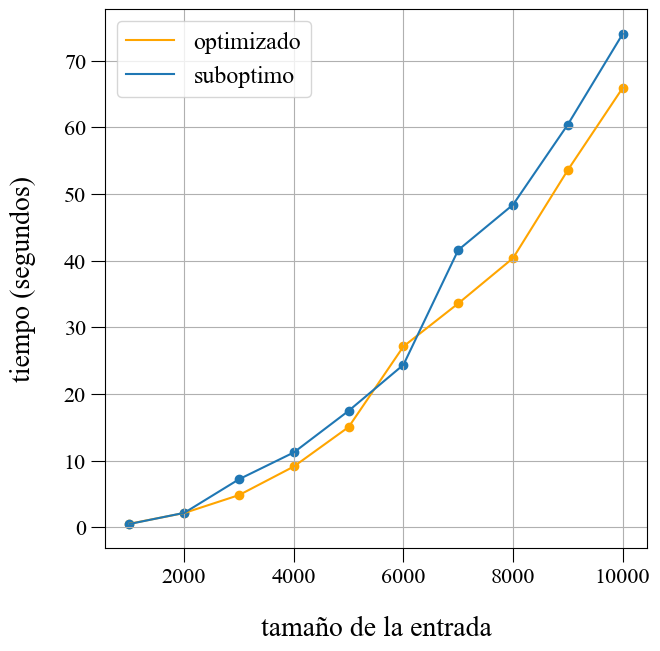
\includegraphics[scale=0.4, clip]{./files/src/.media/comparacion_DSU.png}
    \caption{Tiempo de ejecución del \textsc{modems} en función del tamaño de entrada $n$ para el algoritmo supercuadrático \textit{optimizado} ---con las heurísticas--- y \textit{subóptimo} ---o, ingénuo---.}\label{fig2}
\end{figure}

Notamos que, en general, la versión con las heurísticas parece funcionar mejor. Esto puede deberse a las constantes \textit{invisibles} asociadas a cada algoritmo, ya que $\Theta(n^2) < \Theta(m\alpha(n))$ si el grafo de entrada es \textit{denso}. Es decir, cuando $m \approx n^2$. 

\newpage

% apendice
% \section{Apéndice}
% \input{files/src/apendice.tex}
% \newpage

%bibliografia - requiere que haya citas
% \bibliographystyle{plain}
% \bibliography{./files/citations.bib}
% \newpage

\end{document}
